%%% NORDIC PGDAY 2018
%%%
%%% Data Modeling, Normalization and Denormalization
%%%
%%% As a developer using PostgreSQL one of the most important tasks you have
%%% to deal with is modeling the database schema for your application. In
%%% order to achieve a solid design, it’s important to understand how the
%%% schema is then going to be used as well as the trade-offs it involves.
%%%
%%% As Fred Brooks said: “Show me your flowcharts and conceal your tables,
%%% and I shall continue to be mystified. Show me your tables, and I won’t
%%% usually need your flowcharts; they’ll be obvious.”
%%%
%%% In this talk we're going to see practical normalisation examples and
%%% their benefits, and also review some anti-patterns and their typical
%%% PostgreSQL solutions, including Denormalization techniques thanks to
%%% advanced Data Types.

\documentclass[xcolor=dvipsnames]{beamer}

\usepackage{minted}

\usepackage{beamerthemesplit}
\usepackage[utf8]{inputenc}
\usepackage[T1]{fontenc}
\usepackage[english]{babel}
\usepackage{calligra}
%% \usepackage{cfr-lm}
\usepackage{tikz}

%% \usepackage{xcolor}

\usepackage{pifont}
\usepackage{newunicodechar}
\newunicodechar{✓}{\ding{51}}
\newunicodechar{✗}{\ding{55}}

\usepackage{csquotes}
\usepackage{ragged2e}

\usetheme{Boadilla}
\setbeamertemplate{itemize items}[square]
\setbeamertemplate{enumerate items}[square]
%\setbeamertemplate{itemize items}{\checkmark}
\beamertemplatenavigationsymbolsempty

\usebackgroundtemplate%
{%
    \begin{tikzpicture}[remember picture,overlay]
      \node[opacity=0.5] at (current page.center) {
        
\includegraphics[width=\paperwidth,height=\paperheight]{mammoth-bg.png}%
      };
    \end{tikzpicture}
}

\title{Data Modeling, Normalization and Denormalization}
\subtitle{Nordic PgDay 2018, Oslo}
\author{Dimitri Fontaine}
\institute{CitusData}
\date{March 13, 2018}
%\logo{
\includegraphics[height=0.4cm]{logo.png}}

\addtobeamertemplate{frametitle}{}{%
\begin{tikzpicture}[remember picture,overlay]
  \node[anchor=north east,yshift=-6pt] at (current page.north east) {
    
\includegraphics[height=0.4cm]{logo-r.png}
  };
\end{tikzpicture}}

%\setbeamercolor{frametitle}{bg=beamer@blendedblue!30}

\begin{document}

\section{Introduction}

\frame{\titlepage}

\begin{frame}[fragile]
  \frametitle{Data Modeling, Normalization and Denormalization}

  \begin{center}
    %% {\Huge Dimitri Fontaine}
    {\textcalligra{\Huge Dimitri Fontaine}}
    \vfill
    {\Large \textbf{PostgreSQL Major Contributor}}
  \end{center}

\begin{columns}[c]
\column{.5\textwidth} 

  \begin{itemize}
   \item \textbf{pgloader}
   \item \texttt{\textbf{CREATE EXTENSION}}
   \item \texttt{\textbf{CREATE EVENT TRIGGER}}
   \item \textit{Bi-Directional Réplication}
   \item \textit{apt.postgresql.org}
  \end{itemize}  

\column{.5\textwidth}
\begin{center}
  
\includegraphics[height=6em]{postgres-logo.png}
\end{center}
\end{columns}
\end{frame}

\begin{frame}
  \frametitle{Mastering PostgreSQL in Application Development}

  \begin{columns}[c]
    \column{.5\textwidth}
    \begin{minipage}[t][12em][t]{\textwidth}
      \begin{center}
        {\textcalligra{\Huge I wrote a book!}}
      \end{center}
      
      \vfill
      
      \textit{Mastering PostgreSQL in Application Development} teaches SQL
      to developpers: learn to replace thousands of lines of code with
      simple queries.

      \vfill
      \url{http://MasteringPostgreSQL.com}
    \end{minipage}

    \column{.5\textwidth} 
    \begin{center}
      \href{http://MasteringPostgreSQL.com}
           {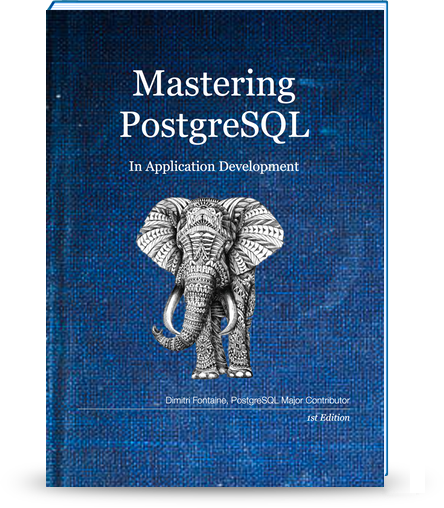
\includegraphics[height=18em]{MasteringPostgreSQLinAppDev-Cover.png}}
    \end{center}
  \end{columns}
\end{frame}

{
  \usebackgroundtemplate{
    \begin{tikzpicture}[remember picture,overlay]
      \node[opacity=0.25] at (current page.center) {
        %
\includegraphics{darpa_wallpaper.jpg}
        \includegraphics{data-analysis.png}
      };
    \end{tikzpicture}
  }
 
  \begin{frame}
    \frametitle{Rob Pike, Notes on Programming in C}

    \begin{center}
      \textbf{\Large \texttt{Rule 5.} \textit{Data dominates.}}
    \end{center}

    \vfill

    \begin{displayquote}[Brooks p. 102.]
     \LARGE If you've chosen the right data structures and organized things
     well, the algorithms will almost always be self-evident. Data
     structures, not algorithms, are central to programming.
    \end{displayquote}

    \vfill
  \end{frame}
}

{
  \usebackgroundtemplate{
    \begin{tikzpicture}[remember picture,overlay]
      \node[opacity=0.2] at (current page.center) {
        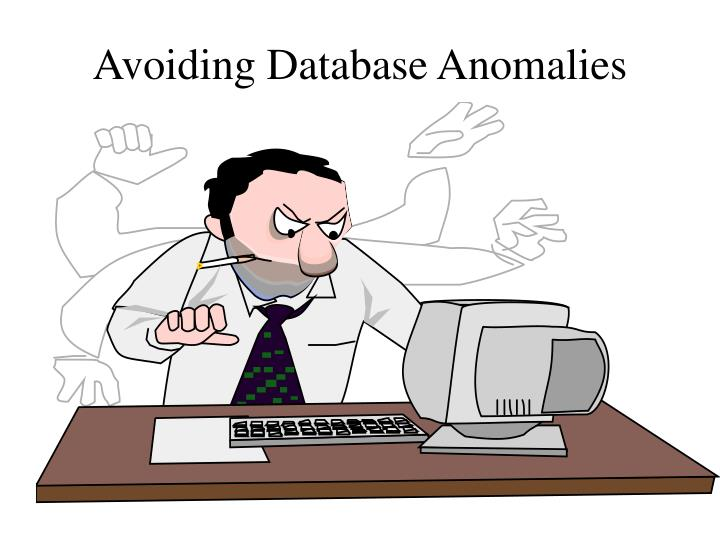
\includegraphics[width=\paperwidth,height=\paperheight]
                        {avoiding-database-anomalies-n.jpg}
      };
    \end{tikzpicture}
  }
 
  \begin{frame}[fragile]
    \frametitle{Database Anomalies}

    We normalize a database model so as to avoid \textit{Database Anomalies}.
    We also follow simple data structure design rules to make the data easy to
    understand, maintain and query.

    \vfill
    
    \begin{columns}[c]
      \column{.5\textwidth}
      Database Anomalies

      \begin{itemize}
      \item Update anomaly
      \item Insertion anomaly
      \item Deletion anomaly
      \end{itemize}
      
    \end{columns}
  \end{frame}
}

\begin{frame}
  \frametitle{Update Anomaly}

  \begin{center}
    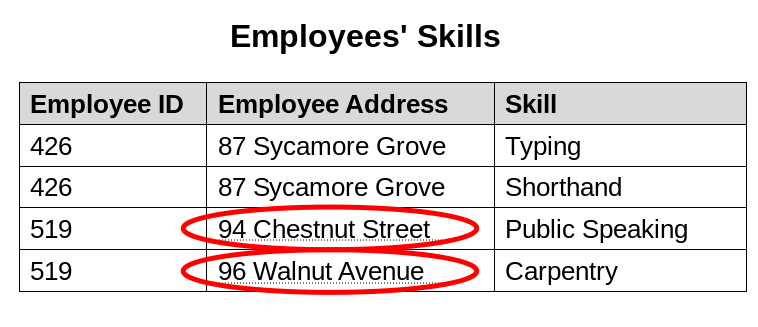
\includegraphics[width=0.8\paperwidth]{Update_anomaly.png}
  \end{center}
\end{frame}

\begin{frame}
  \frametitle{Insertion Anomaly}

  \begin{center}
    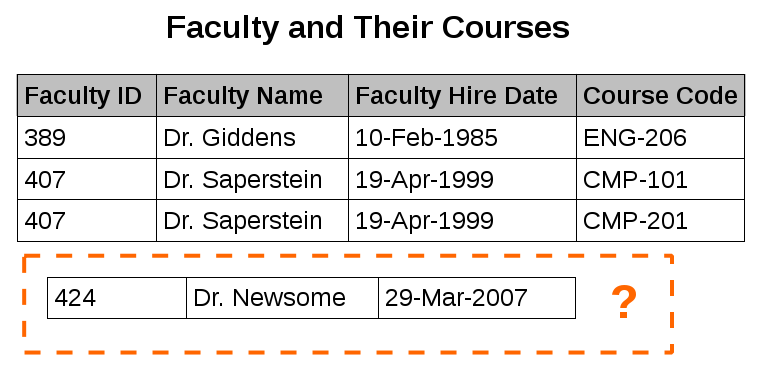
\includegraphics[width=0.8\paperwidth]{Insertion_anomaly.png}
  \end{center}
\end{frame}

\begin{frame}
  \frametitle{Deletion Anomaly}

  \begin{center}
    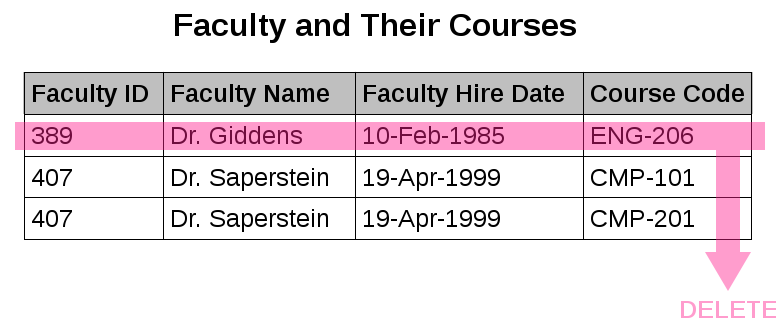
\includegraphics[width=0.8\paperwidth]{Deletion_anomaly.png}
  \end{center}
\end{frame}

{
  \usebackgroundtemplate{
    \begin{tikzpicture}[remember picture,overlay]
      \node[opacity=0.25] at (current page.center) {
        %
\includegraphics{darpa_wallpaper.jpg}
        \includegraphics{data-analysis.png}
      };
    \end{tikzpicture}
  }
 
  \begin{frame}
    \frametitle{Database Design and User Workflow}

    \begin{displayquote}[Fred Brooks]
     \LARGE Show me your flowcharts and conceal your tables, and I shall
     continue to be mystified. Show me your tables, and I won’t usually need
     your flowcharts; they’ll be obvious.
    \end{displayquote}

    \vfill
  \end{frame}
}

\section{Tooling}

{
  \usebackgroundtemplate{
    \begin{tikzpicture}[remember picture,overlay]
      \node[opacity=0.4] at (current page.center) {
        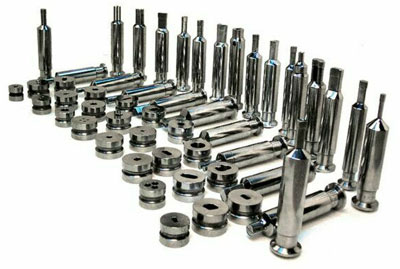
\includegraphics[width=\paperwidth,height=\paperheight]{tooling.jpg}
      };
    \end{tikzpicture}
  }
 
  \begin{frame}
    \frametitle{Database Modeling \& Tooling}
  \end{frame}
}
    
    

\begin{frame}[fragile]
  \frametitle{Tooling for Database Modeling}

  We can use \texttt{psql} and SQL scripts to edit database schemas:
  
  \begin{minted}
    [frame=lines,bgcolor=beamer@blendedblue!10,linenos,fontsize=\small]
    {plpgsql}
BEGIN;

create schema if not exists sandbox;

create table sandbox.category
 (
   id    serial primary key,
   name  text not null
 );

insert into sandbox.category(name)
     values ('sport'),('news'),('box office'),('music');

ROLLBACK;
    \end{minted}
\end{frame}

{
  \usebackgroundtemplate{
    \begin{tikzpicture}[remember picture,overlay]
      \node[opacity=0.25] at (current page.center) {
        %%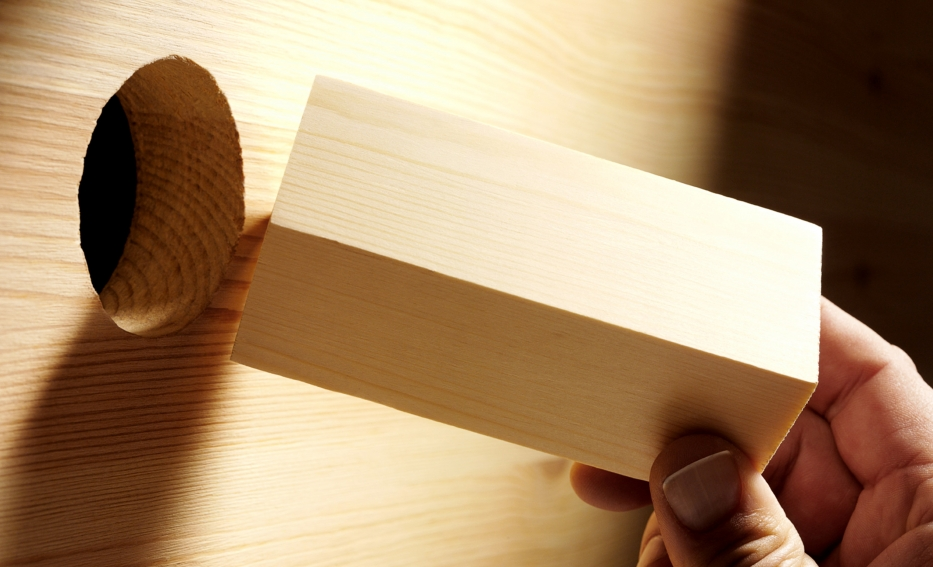
\includegraphics{square_round.jpg}
        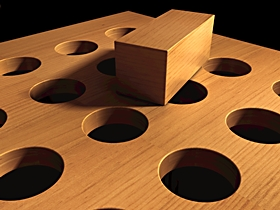
\includegraphics[scale=1.5]{Square_peg_round_hole.jpg}
      };
    \end{tikzpicture}
  }
 
  \begin{frame}
    \frametitle{Object Relational Mapping}

    The R in \textbf{ORM} stands for \textit{“Relation”}. The result of a
    SQL query is a relation. That's what you should be mapping, not your
    base tables! \vfill

    When mapping base tables, you end up trying to solve different complex
    issues at the same time:
    
    \begin{itemize}
    \item User Workflow
    \item Consistent view of the whole world at all time
    \end{itemize}

  \end{frame}
}


\section{Normalization}

{
  \usebackgroundtemplate{
    \begin{tikzpicture}[remember picture,overlay]
      \node[opacity=1] at (current page.center) {
        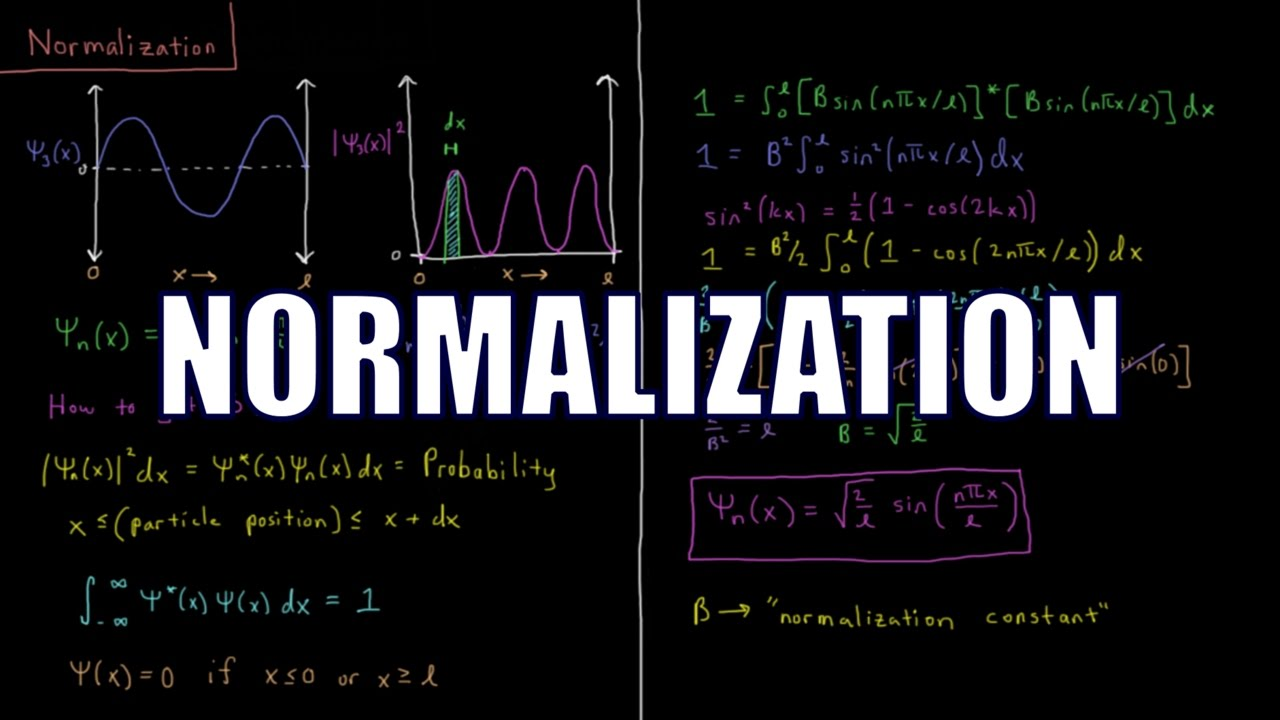
\includegraphics[scale=0.37]{maxresdefault.jpg}
      };
    \end{tikzpicture}
  }
 
  \begin{frame}
  \end{frame}
}

\begin{frame}[fragile]
  \frametitle{Basics of the Unix Philosophy: principles}

  Some design rules that apply to Unix and to database design too:
  
  \begin{itemize}
  \item Rule of Clarity \\
    \textit{Clarity is better than cleverness.}
  \item Rule of Simplicity \\
    \textit{Design for simplicity; add complexity only where you must.}
  \item Rule of Transparency \\
    \textit{Design for visibility to make inspection and debugging easier.}
  \item Rule of Robustness \\
    \textit{Robustness is the child of transparency and simplicity.}
  \end{itemize}
\end{frame}

\begin{frame}[fragile]
  \frametitle{Normal Forms}

  The Normal Forms are designed to avoid database anomalies, and they help
  in following the listed rules seen before.

  \vfill

  \center{\Large 1st Normal Form, Codd, 1970}

  \vfill

  \begin{enumerate}
  \item There are no duplicated rows in the table.
  \item Each cell is single-valued (no repeating groups or arrays).
  \item Entries in a column (field) are of the same kind.
  \end{enumerate}  
\end{frame}

\begin{frame}[fragile]
  \frametitle{Second Normal Form}

  \begin{center}
    {\Large 2nd Normal Form, Codd, 1971}
  \end{center}

  \vfill
  
  A table is in \textit{\Large 2NF} if it is in \textit{\Large 1NF} and if
  all non-key attributes are dependent on all of the key. Since a partial
  dependency occurs when a non-key attribute is dependent on only a part of
  the composite key, the definition of \textit{2NF} is sometimes phrased as:
  
  \vfill
  
  “A table is in \textit{2NF} if it is in \textit{1NF} and if it has no
  partial dependencies.”
\end{frame}

\begin{frame}[fragile]
  \frametitle{Third Normal Form and Boyce-Codd Normal Form}

  \begin{center}
    {\Large 3rd Normal Form (Codd, 1971) \\ and BCNF (Boyce and Codd, 1974)}
  \end{center}

  \begin{columns}[c]
    \column{.5\textwidth}

    \textit{\Large 3NF} A table is in 3NF if it is in 2NF and if it has no
    transitive dependencies.

    \column{.5\textwidth}

    \textit{\Large BCNF} A table is in BCNF if it is in 3NF and if every
    determinant is a candidate key.
  \end{columns}  
\end{frame}

\begin{frame}[fragile]
  \frametitle{More Normal Forms!}

  \center{Each level builds on the previous one.}
  \vfill

  \begin{itemize}
  \item \textit{\Large 4NF} A table is in 4NF if it is in BCNF and if it has
    no multi-valued dependencies.
    \newline

  \item \textit{\Large 5NF} A table is in 5NF, also called “Projection-join
    Normal Form” (PJNF), if it is in 4NF and if every join dependency in the
    table is a consequence of the candidate keys of the table.
    \newline
    
   \item \textit{\Large DKNF} A table is in DKNF if every constraint on the
     table is a logical consequence of the definition of keys and domains.
  \end{itemize}
\end{frame}

{
  \usebackgroundtemplate{
    \begin{tikzpicture}[remember picture,overlay]
      \node[opacity=0.25] at (current page.center) {
         
\includegraphics[width=\paperwidth,height=\paperheight]{db.jpg}
      };
    \end{tikzpicture}
  }
 
  \begin{frame}
    \frametitle{Database Constraints}

    \center{\Large Primary Keys, Surrogate Keys, Foreign Keys, and more…}
  \end{frame}
}


\begin{frame}[fragile]
  \frametitle{Primary Keys}

  First Normal Form requires no duplicated row. I know, let's use a Primary
  Key!
  \vfill

  \begin{minted}
    [frame=lines,bgcolor=beamer@blendedblue!10,linenos,fontsize=\small]
    {plpgsql}
create table sandbox.article
 (
   id         bigserial primary key,
   category   integer references sandbox.category(id),
   pubdate    timestamptz,
   title      text not null,
   content    text
 );
    \end{minted}
\end{frame}

\begin{frame}[fragile]
  \frametitle{Primary Keys, Surrogate Keys}

  Artificially generated key is named a \textit{\Large surrogate key}
  because it is a substitute for \textit{\Large natural key}. A
  \textit{\Large natural key} would allow preventing duplicate entries in
  our data set.
  \vfill
  
  \begin{minted}
    [frame=lines,bgcolor=beamer@blendedblue!10,linenos,fontsize=\small]
    {plpgsql}
insert into sandbox.article (category, pubdate, title)
     values (2, now(), 'Hot from the Press'),
            (2, now(), 'Hot from the Press')
  returning *;
    \end{minted}
\end{frame}

\begin{frame}[fragile]
  \frametitle{Primary Keys, Surrogate Keys}

  \center{Oops.}
  \vfill
  
  \begin{minted}
    [frame=lines,bgcolor=beamer@blendedblue!10,linenos,fontsize=\small]
    {plpgsql}
-[ RECORD 1 ]---------------------------
id       | 3
category | 2
pubdate  | 2018-03-12 15:15:02.384105+01
title    | Hot from the Press
content  | 
-[ RECORD 2 ]---------------------------
id       | 4
category | 2
pubdate  | 2018-03-12 15:15:02.384105+01
title    | Hot from the Press
content  | 

INSERT 0 2
    \end{minted}
\end{frame}

\begin{frame}[fragile]
  \frametitle{Primary Keys, Surrogate Keys}

  Fixing the model is easy enough: implement a \textit{\Large natural
    primary key}.
  
  \vfill
  
  \begin{minted}
    [frame=lines,bgcolor=beamer@blendedblue!10,linenos,fontsize=\small]
    {plpgsql}
create table sandboxpk.article
 (
   category   integer references sandbox.category(id),
   pubdate    timestamptz,
   title      text not null,
   content    text,
   
   primary key(category, pubdate, title)
 );
    \end{minted}
\end{frame}

\begin{frame}[fragile]
  \frametitle{Primary Keys, Foreign Keys}

  Now we have to reference the whole natural key everywhere:
  \vfill

  \begin{minted}
    [frame=lines,bgcolor=beamer@blendedblue!10,linenos,fontsize=\small]
    {plpgsql}
create table sandboxpk.comment
 (
   a_category integer     not null,
   a_pubdate  timestamptz not null,
   a_title    text        not null,
   pubdate    timestamptz,
   content    text,
   
   primary key(a_category, a_pubdate, a_title, pubdate, content),

   foreign key(a_category, a_pubdate, a_title)
    references sandboxpk.article(category, pubdate, title)
 );
    \end{minted}
\end{frame}

\begin{frame}[fragile]
  \frametitle{Primary Keys, Foreign Keys}

  One solution is to have both a surrogate and a natural key:
  \vfill
  
  \begin{minted}
    [frame=lines,bgcolor=beamer@blendedblue!10,linenos,fontsize=\small]
    {plpgsql}
create table sandbox.article
 (
   id         integer      generated always as identity,
   category   integer      not null references sandbox.category(id),
   pubdate    timestamptz  not null,
   title      text         not null,
   content    text,

   primary key(category, pubdate, title),
   unique(id)
 );
    \end{minted}
\end{frame}


\begin{frame}[fragile]
  \frametitle{Normalization Helpers: database constraints}

  To help you implement Normal Forms with strong guarantees even when having
  to deal with concurrent access to the database, we have \textit{\Large
    constraints}.

  \begin{columns}[c]
    \column{.5\textwidth}
    \begin{itemize}
    \item Primary Keys
    \item Foreign Keys
    \item Not Null
    \item Check Constraints
    \item Domains
    \item Exclusion Constraints
    \end{itemize}
    \column{.5\textwidth}
    \begin{minted}
      [frame=lines,bgcolor=beamer@blendedblue!10,linenos,fontsize=\small]
      {plpgsql}
create table rates
 (
  currency text,
  validity daterange,
  rate     numeric,

  exclude using gist
  (
     currency with =,
     validity with &&
  )
 );
  \end{minted}    
  \end{columns}  
\end{frame}


%\section{Normalization Anti-Patterns}

\section{Denormalization}

\begin{frame}[fragile]
  \frametitle{Denormalization}

  \begin{center}
    
\includegraphics{optimisation_rules.jpg}
  \end{center}
\end{frame}


\begin{frame}[fragile]
  \frametitle{Denormalization}

  \begin{center}
    {\Huge The first rule \\
    of denormalization is that you \\
    \textbf{don't} \\
    do denormalization.
    }
  \end{center} 
\end{frame}

\begin{frame}[fragile]
  \frametitle{Denormalization is an optimization technique}
  
  \begin{displayquote}
    Programmers waste enormous amounts of time thinking about, or worrying
    about, the speed of noncritical parts of their programs, and these
    attempts at efficiency actually have a strong negative impact when
    debugging and maintenance are considered. We should forget about small
    efficiencies, say about 97\% of the time: {\Huge premature optimization
      is the root of all evil.} Yet we should not pass up our opportunities
    in that critical 3\%.
  \end{displayquote}

  \textbf{Donald Knuth}, \textit{"Structured Programming with Goto
    Statements". Computing Surveys 6:4 (December 1974), pp. 261–301, §1.}
\end{frame}

\begin{frame}[fragile]
  \frametitle{Denormalization: cache data}

  The main trick: repeat data to make it locally available, breaking
  functional dependency rules. You know have a cache.
  \vfill

  \begin{center}
    Implement {\LARGE Cache Invalidation}.
  \end{center}
\end{frame}

\begin{frame}[fragile]
  \frametitle{Denormalization example}

  \begin{minted}
    [frame=lines,bgcolor=beamer@blendedblue!10,linenos,fontsize=\small]
    {plpgsql}
\set season 2017

  select drivers.surname as driver,
         constructors.name as constructor,
         sum(points) as points
    
    from results
         join races using(raceid)
         join drivers using(driverid)
         join constructors using(constructorid)
   
   where races.year = :season

group by grouping sets(drivers.surname, constructors.name)
  having sum(points) > 150
order by drivers.surname is not null, points desc;
  \end{minted}    
\end{frame}


\begin{frame}[fragile]
  \frametitle{Denormalization example}

  \begin{minted}
    [frame=lines,bgcolor=beamer@blendedblue!10,linenos,fontsize=\small]
    {plpgsql}
create view v.season_points as
  select year as season, driver, constructor, points
    from seasons left join lateral
         (
            select drivers.surname as driver,
                   constructors.name as constructor,
                   sum(points) as points
              from results
                   join races using(raceid)
                   join drivers using(driverid)
                   join constructors using(constructorid)
             where races.year = seasons.year
          group by grouping sets(drivers.surname, constructors.name)
          order by drivers.surname is not null, points desc
          )
          as points on true
order by year, driver is null, points desc;
  \end{minted}    
\end{frame}


\begin{frame}[fragile]
  \frametitle{Denormalization example}

  And now cache the results of the view into a durable relation:
  
  \begin{minted}
    [frame=lines,bgcolor=beamer@blendedblue!10,linenos,fontsize=\small]
    {plpgsql}
create materialized view cache.season_points as
  select * from v.season_points;

create index on cache.season_points(season);
  \end{minted}

  \vfill

  When you need to invalidate the cache, just {\Large refresh} the view:

  \begin{minted}
    [frame=lines,bgcolor=beamer@blendedblue!10,linenos,fontsize=\small]
    {plpgsql}
  refresh materialized view cache.season_points;
  \end{minted}

\end{frame}


\begin{frame}[fragile]
  \frametitle{Denormalization example}

  And now rewrite your application's query as:
  \vfill
  
  \begin{minted}
    [frame=lines,bgcolor=beamer@blendedblue!10,linenos,fontsize=\small]
    {plpgsql}
select driver, constructor, points
  from cache.season_points
 where season = 2017
   and points > 150;
  \end{minted}

\end{frame}

{
  \usebackgroundtemplate{
    \begin{tikzpicture}[remember picture,overlay]
      \node[opacity=0.25] at (current page.center) {
        
\includegraphics[width=\paperwidth,height=\paperheight]
                        {eoy-audit-blog-big.png}
      };
    \end{tikzpicture}
  }
  
  \begin{frame}[fragile]
    \frametitle{Other denormalization use cases}

    \begin{columns}[c]
      \column{.4\textwidth}
      \begin{itemize}
      \item {\Large Audit Trails}
      \item {\Large History Tables}
      \end{itemize}

      \column{.4\textwidth}
      \begin{itemize}
      \item {\Large Partitionning}
      \item {\Large Scaling Out}
      \end{itemize}
    \end{columns}
  \end{frame}
}


\begin{frame}[fragile]
  \frametitle{History tables and audit trails}

  Another case where you might have to denormalize your database model is
  when keeping a history of all changes.
  \vfill

  \begin{itemize}
  \item
    Foreign key references to other tables won't be possible when those
    reference changes and you want to keep a history that, by definition,
    doesn't change.
    \newline
    
  \item
    The schema of your main table evolves and the history table shouldn't
    rewrite the history for rows already written.
  \end{itemize}
\end{frame}

\begin{frame}[fragile]
  \frametitle{History tables with JSONB}

  JSONB is very flexible, and can host the archives for all your database
  model versions in the same table, or for all your source tables at once
  even.
  \vfill

  \begin{minted}
    [frame=lines,bgcolor=beamer@blendedblue!10,linenos,fontsize=\small]
    {plpgsql}
create schema if not exists archive;

create type archive.action_t
    as enum('insert', 'update', 'delete');

create table archive.older_versions
 (
   table_name text,
   date       timestamptz default now(),
   action     archive.action_t,
   data       jsonb
 );
   \end{minted}
\end{frame}


\begin{frame}[fragile]
  \frametitle{Validity periods}

  A variant of the historic requirement is to keep track of data changes and
  be able to use the value that were valid at a known time. Currency
  exchange rates applied to invoices is an example:
  \vfill

  \begin{minted}
    [frame=lines,bgcolor=beamer@blendedblue!10,linenos,fontsize=\small]
    {plpgsql}
create table rates
 (
  currency text,
  validity daterange,
  rate     numeric,

  exclude using gist (currency with =,
                      validity with &&)
 );
   \end{minted}
\end{frame}


\begin{frame}[fragile]
  \frametitle{Validity periods}

  Here's how to use the data from a known time in the past:
  \vfill

  \begin{minted}
    [frame=lines,bgcolor=beamer@blendedblue!10,linenos,fontsize=\small]
    {plpgsql}
  select currency, validity, rate
    from rates
   where currency = 'Euro'
   and validity @> date '2017-05-18';

-[ RECORD 1 ]---------------------
currency | Euro
validity | [2017-05-18,2017-05-19)
rate     | 1.240740
   \end{minted}
\end{frame}

\begin{frame}[fragile]
  \frametitle{Denormalization Helpers: advanced datatypes}

  Composite datatypes help with denormalization. It's possible to keep
  several values in the same column thanks to them. Spare matrix becomes an
  \textit{extra} field of \texttt{jsonb} type.
  \vfill

  \begin{columns}[c]
    \column{.1\textwidth}
    \column{.4\textwidth}
    \begin{itemize}
    \item Composite Types
    \item Arrays
    \item JSONb
    \item Enumerated Types
    \end{itemize}
    \column{.4\textwidth}
    \begin{itemize}
    \item \texttt{hstore}
    \item \texttt{ltree}
    \item \texttt{intarray}
    \item \texttt{pg\_trgm}
    \end{itemize}
  \end{columns}  
\end{frame}

\begin{frame}[fragile]
  \frametitle{Partitioning}

  Partitioning comes with demormalization trade-offs in PostgreSQL 10:
  \vfill

  \begin{itemize}
    \item Index are managed at the partition level
    \item No Primary Key, No Unique Index, No Exclusion Constraint
    \item No Foreign Key pointing to a partitionned table
    \item Lack of \texttt{ON CONFLICT} support
    \item Lack of \texttt{UPDATE} support for \textit{re-balancing}
  \end{itemize}
\end{frame}

\section{Not Only SQL}

\begin{frame}[fragile]
  \frametitle{Not Only SQL}

  \begin{center}
    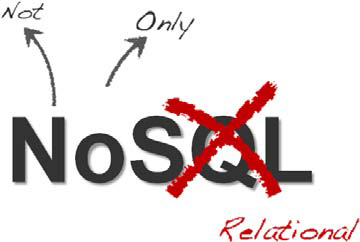
\includegraphics{nosql-1.jpg}
  \end{center}
\end{frame}

{
  \usebackgroundtemplate{
    \begin{tikzpicture}[remember picture,overlay]
      \node[opacity=0.45] at (current page.center) {
        
\includegraphics[height=\paperheight]
                        {1200px-JSON_vector_logo.png}
      };
    \end{tikzpicture}
  }

  \begin{frame}[fragile]
    \frametitle{Schemaless design}

    PostgreSQL includes several composite types (multi-value data). JSONb
    allows the implementation of schemaless design right within PostgreSQL.
    \vfill

  \begin{minted}
    [frame=lines,bgcolor=beamer@blendedblue!10,linenos,fontsize=\small]
    {plpgsql}
select jsonb_pretty(data)
  from magic.cards
 where data @> '{"type":"Enchantment",
                 "artist":"Jim Murray",
                 "colors":["White"]
                }';
   \end{minted}
    
  \end{frame}
}

\begin{frame}[fragile]
  \frametitle{NoSQL and Durability Trade-Offs}

  PostgreSQL setup is made with GUC, or \textit{Great Unified
    Configuration}. You can edit values in the \texttt{postgresql.conf}
  file, or dynamically change it in the session. Or in the transaction
  with \texttt{SET LOCAL}. Or have per-user or per-database settings.
  \vfill

  \begin{minted}
    [frame=lines,bgcolor=beamer@blendedblue!10,linenos,fontsize=\small]
    {plpgsql}
create role dbowner with login;
create role app with login;

create role critical  with login in role app inherit;
create role notsomuch with login in role app inherit;
create role dontcare  with login in role app inherit;

alter user critical  set synchronous_commit to remote_apply;
alter user notsomuch set synchronous_commit to local;
alter user dontcare  set synchronous_commit to off;
  \end{minted}  
\end{frame}


\begin{frame}[fragile]
  \frametitle{Automatic Per-Transaction Durability Setting}

  \begin{minted}
    [frame=lines,bgcolor=beamer@blendedblue!10,linenos,fontsize=\small]
    {plpgsql}
SET demo.threshold TO 1000;
    
CREATE OR REPLACE FUNCTION public.syncrep_important_delta()
  RETURNS TRIGGER
  LANGUAGE PLpgSQL
AS
$$ DECLARE
  threshold integer := current_setting('demo.threshold')::int;
  delta integer := NEW.abalance - OLD.abalance;
BEGIN
  IF delta > threshold
  THEN
    SET LOCAL synchronous_commit TO on;
  END IF;
  RETURN NEW;
END;
$$;    
  \end{minted}  
\end{frame}

\section{Denormalizing to scale: Sharding}

{
  \usebackgroundtemplate{
    \begin{tikzpicture}[remember picture,overlay]
      \node[opacity=1] at (current page.center) {
        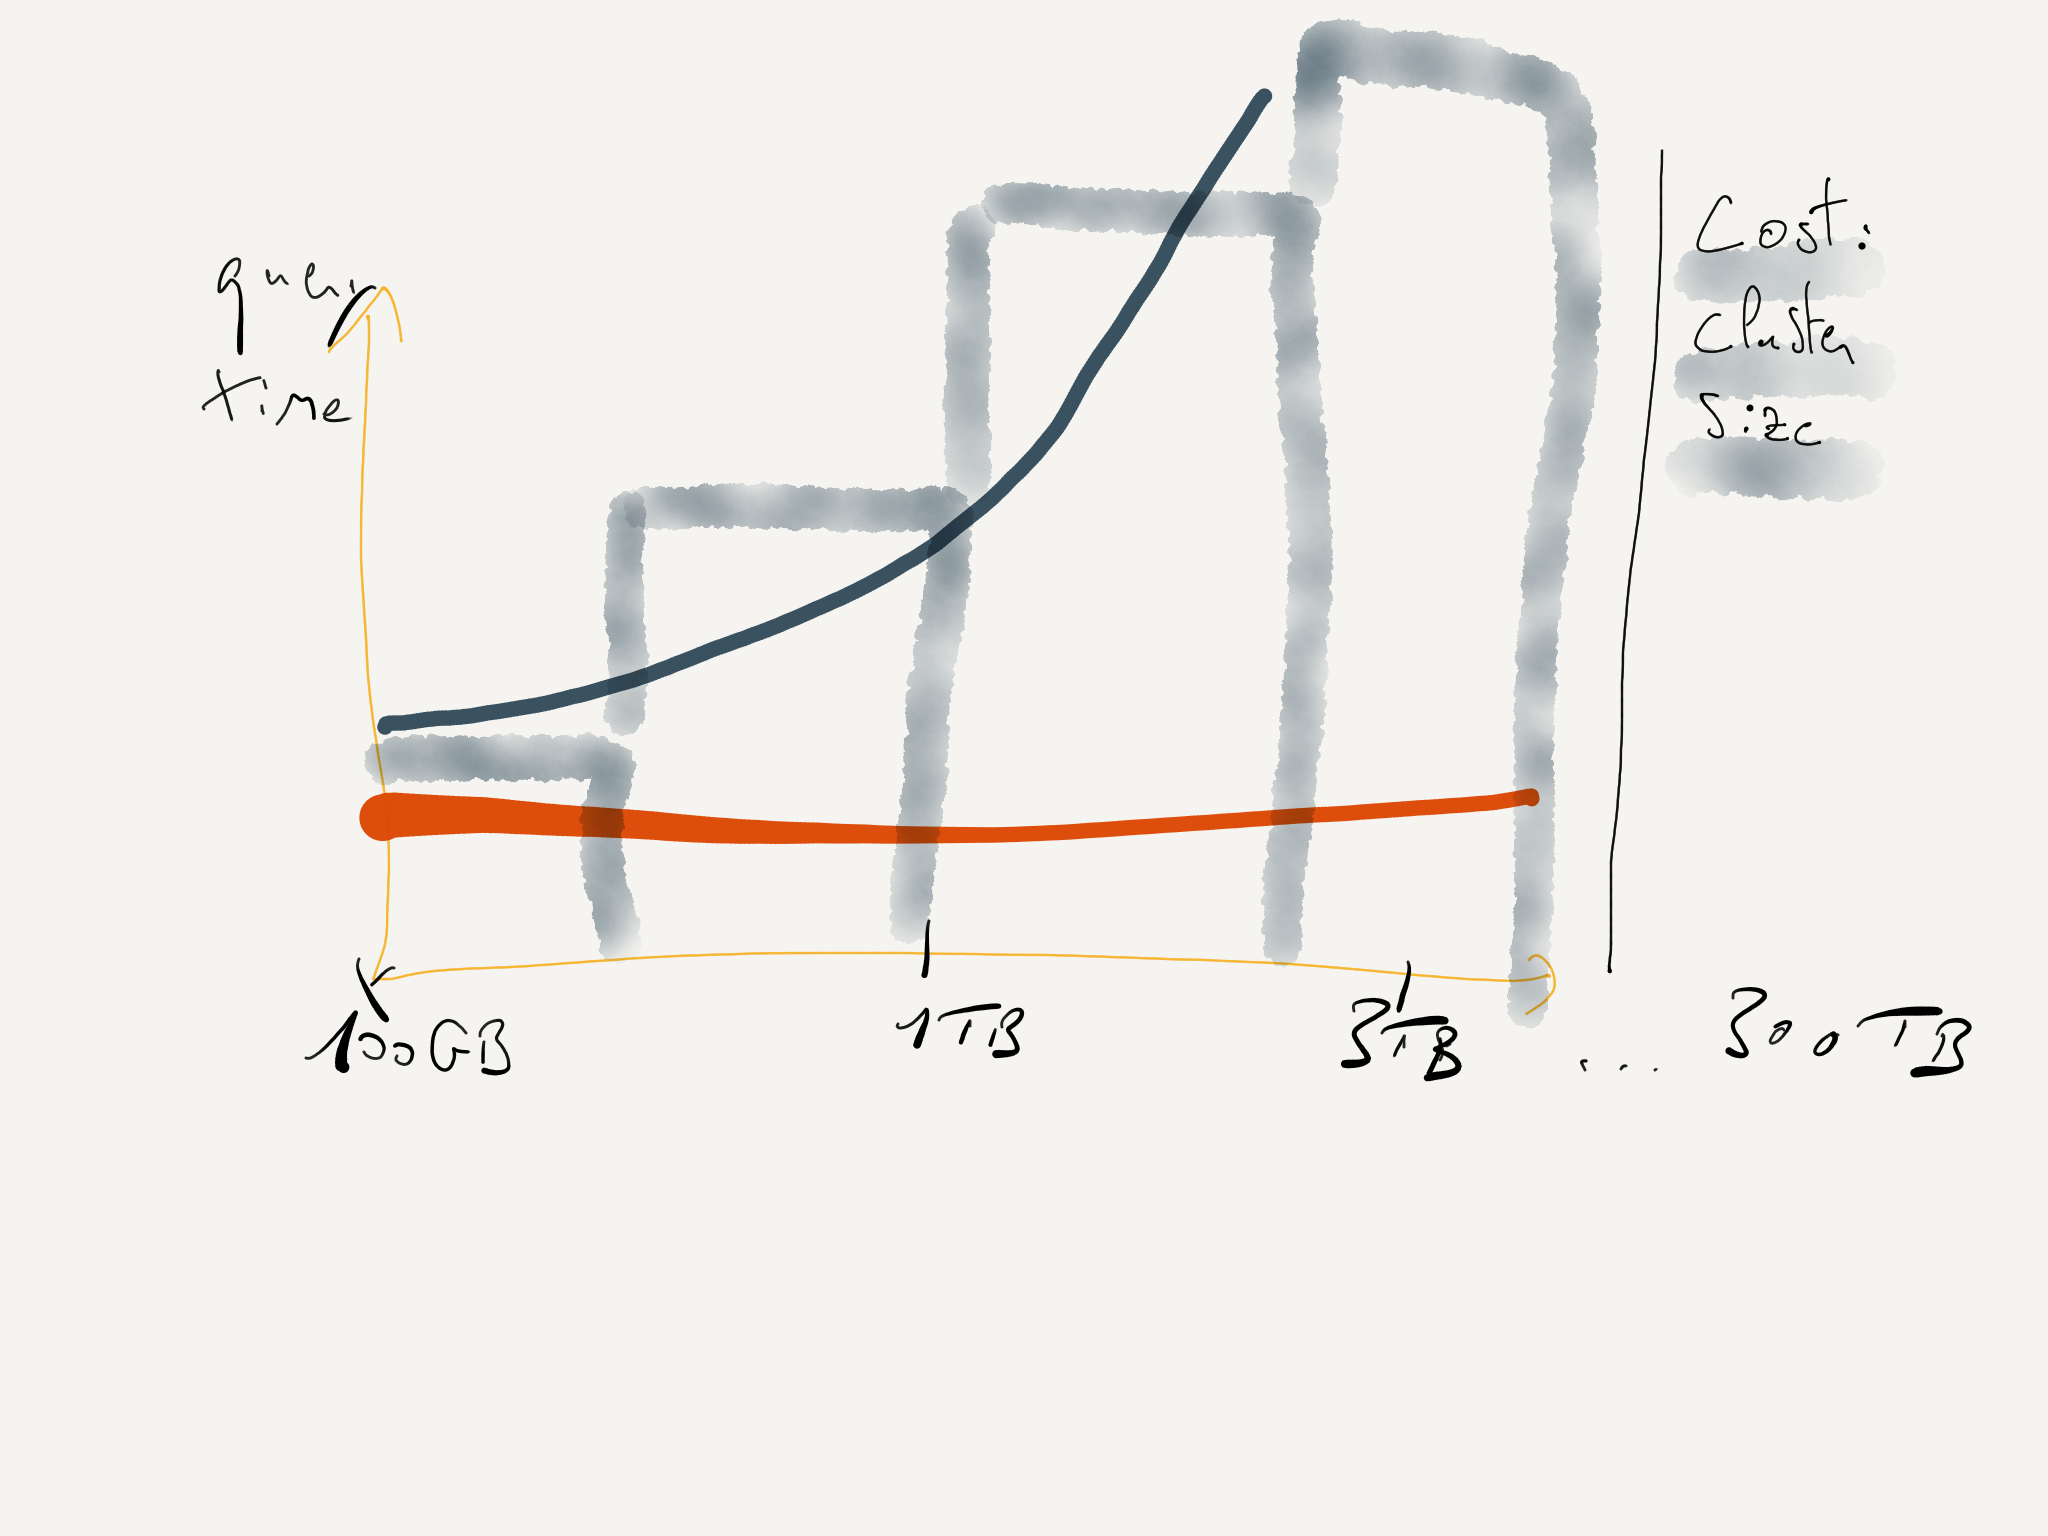
\includegraphics[width=\paperwidth,height=\paperheight]
                        {horizontal-scale.png}
      };
    \end{tikzpicture}
  }

  \begin{frame}[fragile]
    \frametitle{Horizontal Scaling: Sharding}

  \end{frame}
}

{
  \usebackgroundtemplate{
    \begin{tikzpicture}[remember picture,overlay]
      \node[opacity=0.3] at (current page.center) {
        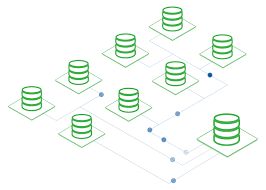
\includegraphics[width=\paperwidth,height=\paperheight]{sharding.png}
      };
    \end{tikzpicture}
  }
  \begin{frame}
    \frametitle{Five sharding data models and which is right?}

    If you were here this morning you've seen Craig's talk, so that's about it.
    \vfill

    \begin{columns}[c]
      \column{.5\textwidth}
      \begin{itemize}
      \item Sharding by geography
      \item Sharding by entity id
      \item Sharding a graph
      \item Time partitioning
      \item Depends…
      \end{itemize}
    \end{columns}

  \end{frame}
}

\begin{frame}[fragile]
  \frametitle{Denormalization and Sharding}

  \begin{columns}[c]
    \column{.6\textwidth}

    {\Large Adding the sharding key to every table is another case of
      \textit{duplicating} information for maintaining a \textbf{\textit{
          cache.}} Beware of \textit{database anomalies}}
  \end{columns}
\end{frame}


{
  \usebackgroundtemplate{
    \begin{tikzpicture}[remember picture,overlay]
      \node[opacity=0.2] at (current page.center) {
        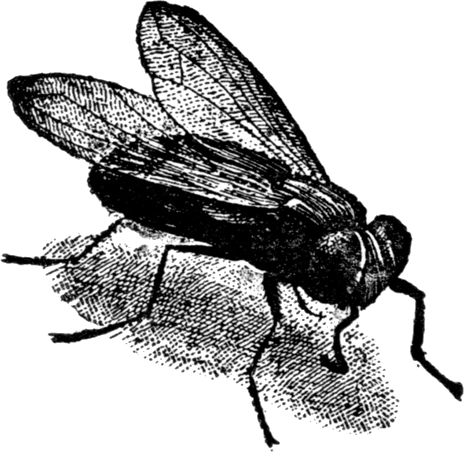
\includegraphics[width=0.8\paperwidth,height=0.8\paperheight]{fly.png}
      };
    \end{tikzpicture}
  }
 
  \begin{frame}
    \frametitle{Questions?}

    \begin{center}
      \textbf{\Large Now is the time to ask!}
      \vfill
      \url{https://2018.nordicpgday.org/feedback}
    \end{center}
  \end{frame}
}

\end{document}
